\documentclass{article}
\usepackage[utf8]{inputenc}
\usepackage{float}
\usepackage{graphicx}
\usepackage{geometry}
\usepackage{tabularx}
\usepackage{acronym}
\usepackage{listings}
\usepackage{lmodern}
\usepackage[version=4]{mhchem}
\usepackage{multicol}
\usepackage{xcolor}

\title{Systems Integration - Assignment \#2}
\date{2019/2020}

\author{João Moreira - 2015230374 \\ 
João Soares - 2009113071 }

\renewcommand{\baselinestretch}{1.3}

\begin{document}

\maketitle

\section{Introduction}

\qquad The intent of this assignment is to develop a web application to manage an online store os secondhand items, called MyBay and deploy it using WildFly Application Server. In order to develop this application, we build a Maven architecture and used \ac{Java EE} and divided the system into three layers: presentation, business and data.

\section{Presentation layer}

\qquad To develop the presentation layer we used \ac{JSF}.

\qquad structure of the webpage -> layout and templates

\begin{figure}[hbt!]
 \centering
 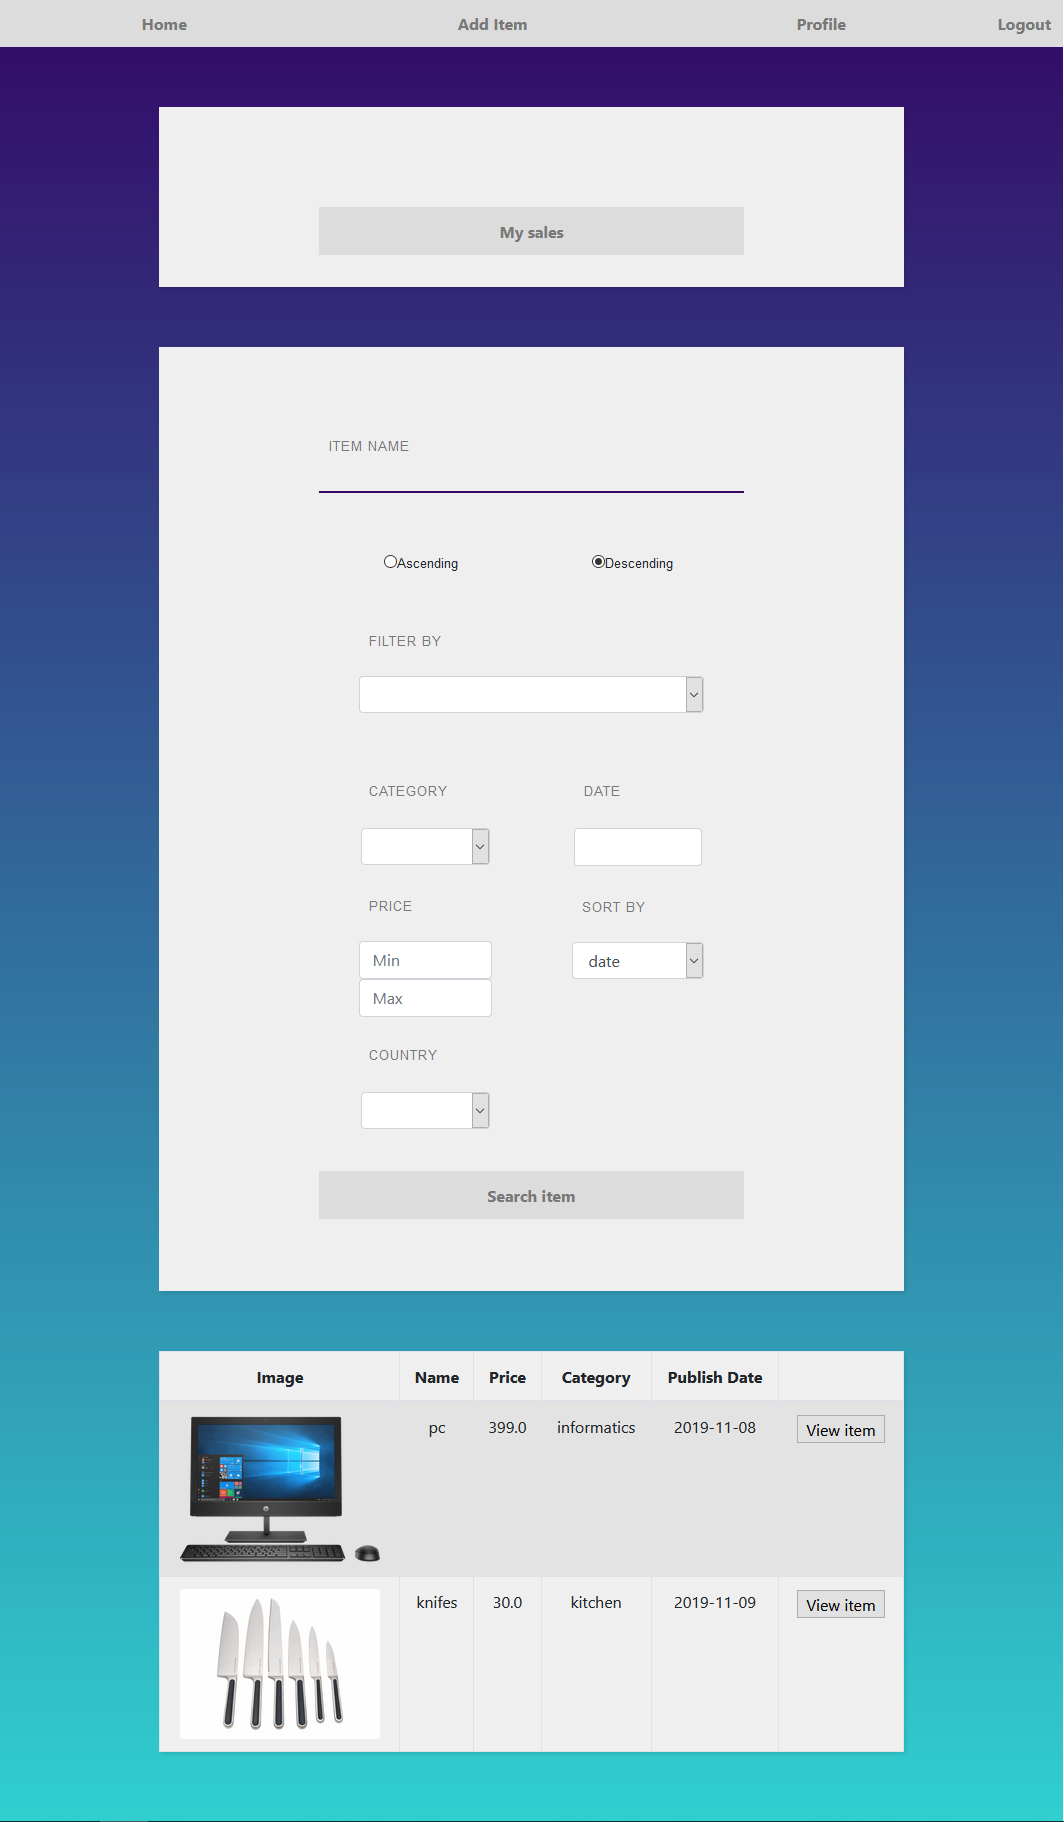
\includegraphics[scale=0.30]{homePage.png}
 \caption{Home page layout }
\end{figure}

\qquad details that were most complex to implement in the interface

\qquad password storage




\section{Business layer}

\qquad This layer interacts with the data layer, built with \ac{EJB}.

\qquad describe the time of ejbs (stateless, interface types, transaction management)

\qquad what data is being transferred from the business layer to the presentation (how)

\qquad what data do we collect from the data layer to the business layer





\section{Data layer}

\qquad This layer works atop a database (postgres) and exposes CRUD functionalities using \ac{EJB}s

\qquad Include ER

\begin{figure}[hbt!]
 \centering
 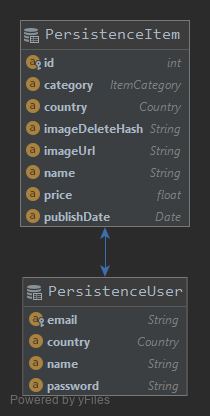
\includegraphics[scale=0.4]{ER_MyBay.png}
 \caption{MyBay \ac{EJB} \ac{ER} diagram }
\end{figure}

\qquad listing of entities






\section{Project management and packaging}

\qquad The logging tool used was \ac{SLF4J}

\qquad description of poms and structure of the project






\textbf{Acronym list:}

\begin{acronym}
\acro{Java EE}{Java Enterprise Edition}
\acro{JSF}{JavaServer Faces}
\acro{EJB}{Enterprise JavaBeans}
\acro{JPA}{Java Persistence API}
\acro{JPQL}{Java Persistence Query Language}
\acro{ORM}{Object/Relational Mapping}
\acro{SLF4J}{Simple Logging Facade for Java}
\acro{ER}{Entity-Relationship}
\end{acronym}

\end{document}
